\documentclass{article}
\usepackage{graphicx}
\usepackage{amsmath}
\usepackage{amssymb}
\usepackage[a4paper, top=25mm, bottom=25mm, left=25mm, right=25mm]{geometry}
\usepackage{pgfplots}
\pgfplotsset{compat=1.18}
\usepackage{mathtools}

\begin{document}
\pagestyle{empty}
\large

\begin{center}
2019-2020 Spring \\MAT124 Midterm\\(08/06/2020)
\end{center}

\noindent 1. Find an equation for the line $L$ that contains the point $P= (-1,3,1)$ and is orthogonal to the line

\[\frac{x-2}{-1}=\frac{y-1}{-2}=\frac{z-5}{1}=\lambda,\quad\lambda\in\mathbb{R}\]

\hfill

\noindent 2. Sketch the graph of the following surfaces.

\hfill

(a) $z=\mathrm e^y$ \ \ \ (b) $y=z^2-x^2$

\hfill

\noindent 3. The position vector for a particle in space is given as

\[\textbf{R}(t) = (2\cos t)\textbf{i}+t^2\textbf{j}+(2\sin t)\textbf{k}.\]
    
\noindent Find the velocity and acceleration vectors of the particle and find the speed and direction of motion at t = $\pi/2$.

\hfill

\noindent 4. Let $f$ be a function defined by

\[
f(x,y) =
\left.
\begin{cases}
\dfrac{xy^3}{x^2+y^6},&\text{if}\, (x, y)\neq (0,0)\\[1em]0,&\text{if}\,(x,y)=(0,0).
\end{cases}
\right.
\]

\hfill

\noindent Is $f$ continuous at $(0,0)$? Explain.

\hfill

\noindent 5. Use the $\epsilon - \delta$ definition and show that the function

\[
f(x,y) =
\left.
\begin{cases}
\displaystyle \frac{x^2y}{x^2+y^6},&\text{if}\, (x, y)\neq (0,0)\\[1em]0,&\text{if}\,(x,y)=(0,0)
\end{cases}
\right.
\]

\hfill

\noindent is continuous at the origin.

\hfill

\noindent 6. Note that in Cartesian coordinates, the Cauchy-Riemann equations are

\[\frac{\partial u}{\partial x}=\frac{\partial v}{\partial y}\quad\text{and}\quad\frac{\partial u}{\partial y}=-\frac{\partial v}{\partial x}\]

\hfill

\noindent where $u=(x,y)$ and $v=v(x,y)$.

\hfill

\noindent Let $x=r\cos\theta$ and $y=r\sin\theta$. Show that the Cauchy-Riemann equations take the form

\[\frac{\partial u}{\partial r} = \frac{1}{r} \frac{\partial v}{\partial\theta} \quad\text{and}\quad\frac1r\frac{\partial u}{\partial\theta}=-\frac{\partial v}{\partial r}.\]

\newpage

\noindent 7. According to Poiseuille’s law, the resistance to the flow of blood offered by a cylindrical blood vessel of radius $r$ and length $x$ is

\[R(x,r) = \frac{cx}{r^4}\]

\hfill

\noindent for a constant $c > 0$. A certain blood vessel in the body is 8 cm long and has a radius of $2$ mm. Estimate the percent change in $R$ when $x$ is increased by $3\%$ and $r$ is decreased by $2\%$.

\hfill

\noindent 8. Find the critical points of $f(x, y)=-x^3+9x-4y^2$ and classify each point as a relative maximum, a relative minimum, or a saddle point.

\newpage

\begin{center}
2019-2020 Spring Midterm (08/06/2020) Solutions\\
(Last update: 28/08/2025 16:57)
\end{center}

\noindent 1. Let $M$ be the line $\dfrac{x-2}{-1}=\dfrac{y-1}{-2}=\dfrac{z-5}{1}=\lambda,\quad\lambda\in\mathbb{R}$. The direction vector of $M$ is $\mathbf u=\left\langle-1,-2,1\right\rangle$.

\hfill

\noindent Let $\mathbf v=\left\langle a,b,c\right\rangle$, where $a,b,c\in\mathbb R$, be the direction vector of $L$. If $M$ and $L$ are orthogonal, the dot product of the direction vectors is zero.

\[\mathbf u\cdot\mathbf v=\left\langle1,-2,1\right\rangle\cdot\left\langle a,b,c\right\rangle=a-2b+c=0\]

\hfill

\noindent $a,b,c$ could be any number with the relation $a-2b+c=0$. Let $a=1,\, b=1$. Then $c=2b-a=2-1=1$. The direction vector $\mathbf v$ is then $\mathbf v=\left\langle1,1,3\right\rangle$.

\hfill

\noindent The parametric equations for a line that passes through the point $P_0(x_0,y_0,z_0)$ is given by
\[\left.\begin{array}{c}
x=x_0+v_1t\\
y=y_0+v_2t\\
z=z_0+v_3t
\end{array}\right\}\quad t\in\mathbb{R}\]

\hfill

\noindent Therefore, using the point $P$, the parametric equations for the line $L$ is

\[\boxed{\left.\begin{array}{l}
x=-1+t\\
y=3+t\\
z=1+3t
\end{array}\right\}\quad t\in\mathbb{R}}\]

\hfill

\noindent 2.

\hfill

\noindent (a)
\begin{center}
    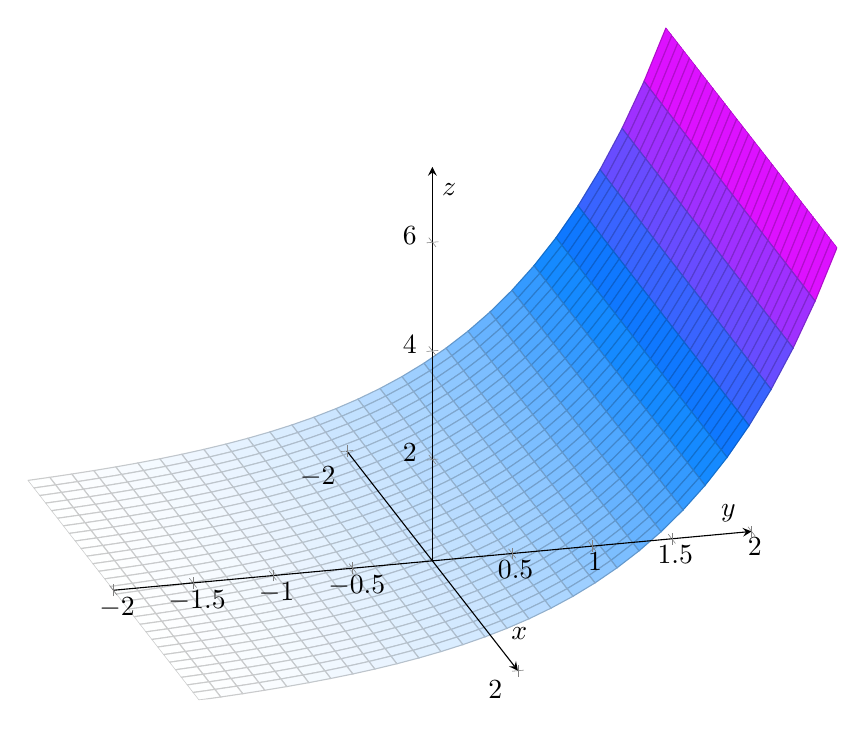
\begin{tikzpicture}
  \begin{axis}[
    view={75}{30},
    axis lines=center,
    xlabel={$x$},
    ylabel={$y$},
    zlabel={$z$},
    domain=-2:2,
    samples=30,
    colormap/cool,
    mesh/ordering=y varies,
    scale=1.5,
    axis on top,
  ]
    \addplot3[surf]  (x, y, {e^y});
  \end{axis}
\end{tikzpicture}
\end{center}

\newpage

\noindent (b)
\begin{center}
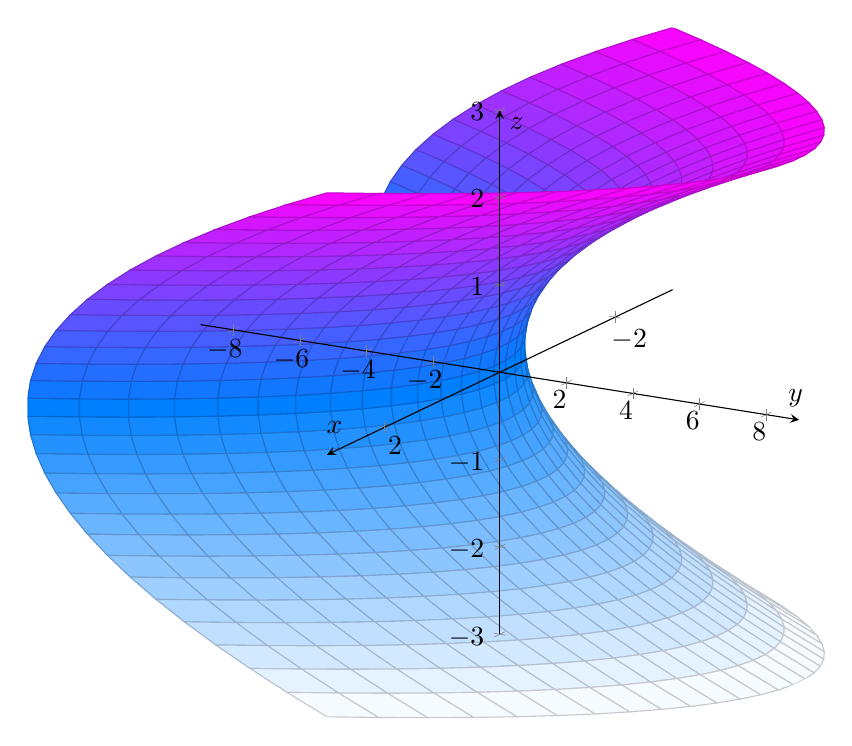
\begin{tikzpicture}
  \begin{axis}[
    view={120}{20},
    axis lines=center,
    xlabel={$x$},
    ylabel={$y$},
    zlabel={$z$},
    domain=-3:3,
    y domain=-3:3,
    samples=30,
    samples y=30,
    colormap/cool,
    z buffer=sort,
    axis on top,
    scale=1.75
  ]
    \addplot3[surf]({x}, {y^2 - x^2}, {y});
  \end{axis}
\end{tikzpicture}
\end{center}

\hfill

\noindent 3. The velocity and acceleration vectors can be obtained by taking the first and the second derivatives of the vector function with respect to the parametrization variable, respectively.

\[\text{Velocity vector}:\mathbf v(t)=\frac{d\mathbf R}{dt}=\left\langle-2\sin t,\,2t,\,2\cos t\right\rangle\]

\[\text{Acceleration vector}:\mathbf a(t)=\frac{d\mathbf v}{dt}=\left\langle-2\cos t,\,2,\,-2\sin t\right\rangle\]

\hfill

\noindent The speed of motion is the magnitude of the velocity vector, and the direction is the normalized velocity vector.

\[\text{Speed}=\left|\mathbf v(t=\pi/2)\right|=\sqrt{\left(-2\sin\frac\pi2\right)^2+\left(2\cdot\frac\pi2\right)^2+\left(2\cos\frac\pi2\right)^2}=\sqrt{4+\pi^2}\]

\[\text{Direction}=\frac{\mathbf v(t=\pi/2)}{\left|\mathbf v(t=\pi/2)\right|}=\frac{\left\langle-2\sin\dfrac\pi2,\,2\cdot\dfrac\pi2,\,2\cos\dfrac\pi2\right\rangle}{\sqrt{4+\pi^2}}=\left\langle-\frac2{\sqrt{4+\pi^2}},\,\frac\pi{\sqrt{4+\pi^2}},0\right\rangle\]

\hfill

\[\boxed{\begin{array}{c}
\mathbf v(t)=\left\langle-2\sin t,\,2t,\,2\cos t\right\rangle\\
\mathbf a(t)=\left\langle-2\cos t,\,2,\,-2\sin t\right\rangle\\[1em]
\text{Speed of motion at }t=\dfrac\pi2:\sqrt{4+\pi^2}\\
\text{Direction of motion at }t=\dfrac\pi2:\left\langle-\dfrac2{\sqrt{4+\pi^2}},\,\dfrac\pi{\sqrt{4+\pi^2}},0\right\rangle\\
\end{array}}\]

\newpage

\noindent 4. Apply the Two-Path Test.

\[x=y\implies\lim_{(x,y)\to(0,0)}\frac{xy^3}{x^2+y^6}=\lim_{y\to0}\frac{y^4}{y^2+y^6}=\lim_{y\to0}\frac{y^2}{1+y^4}=\frac01=0\]
\[x=y^3\implies\lim_{(x,y)\to(0,0)}\frac{xy^3}{x^2+y^6}=\lim_{y\to0}\frac{y^6}{y^6+y^6}=\lim_{y\to0}\frac{y^6}{2y^6}=\frac12\]

\hfill

\noindent Since $0\neq\dfrac12$, by the Two-Path Test, the limit does not exist. Therefore, the function $f$ is not continuous at $(0,0)$.

\hfill

\noindent 5. The value of the function at the point $(0,0)$ is $0$. Therefore, we will show that the limit $L$ is also $0$. For every $\epsilon>0$, there exists a $\delta>0$ such that

\[0<\sqrt{(x-0)^2+(y-0)^2}<\delta\implies\left|f(x,y)-L\right|<\epsilon\]

\begin{align*}\left|\frac{x^2y}{x^2+y^6}-0\right|&=|y|\cdot\left|\frac{x^2}{x^2+y^6}\right|\leq|y|\cdot1=|y|\qquad\left[\frac{x^2}{x^2+y^6}\leq\frac{x^2}{x^2}=1\right]\\\\&\leq|x|+|y|<2\delta\qquad\left[x^2\geq0,\,y^2\geq0,\,\sqrt{x^2+y^2}<\delta\implies|x|<\delta,\,|y|<\delta\right]\end{align*}

\hfill

\noindent Let $\delta=\dfrac\epsilon2$.

\[\left|\frac{x^2y}{x^2+y^6}\right|\leq|x|+|y|=2\cdot\frac\epsilon2=\epsilon\]

\hfill

\noindent Since the limit is equal to the value of the function at $(0,0)$, $f$ is continuous at $(0,0)$.

\hfill

\noindent 6. $u$ and $v$ are functions of $x$ and $y$. $x$ and $y$ are functions of $r$ and $\theta$. Use the chain rule.

\[\frac{\partial u}{\partial r}=\frac{\partial u}{\partial x}\cdot\frac{\partial x}{\partial r}+\frac{\partial u}{\partial y}\cdot\frac{\partial y}{\partial r}=u_x\cdot\cos\theta+u_y\cdot\sin\theta=v_y\cos\theta-v_x\sin\theta\]

\[\frac{\partial v}{\partial\theta}=\frac{\partial v}{\partial x}\cdot\frac{\partial x}{\partial\theta}+\frac{\partial v}{\partial y}\cdot\frac{\partial y}{\partial\theta}\implies\frac1r\frac{\partial v}{\partial\theta}=\frac1r\left(-v_x\cdot r\sin\theta+v_y\cdot r\cos\theta\right)=-v_x\sin\theta+v_y\cos\theta\]

\[\frac{\partial u}{\partial r}=-v_x\sin\theta+v_y\cos\theta=\frac1r\frac{\partial v}{\partial\theta}\]

\hfill

\[\frac{\partial v}{\partial r}=\frac{\partial v}{\partial x}\cdot\frac{\partial x}{\partial r}+\frac{\partial v}{\partial y}\cdot\frac{\partial y}{\partial r}=v_x\cdot\cos\theta+v_y\cdot\sin\theta=-u_y\cos\theta+u_x\sin\theta\]

\[\frac{\partial u}{\partial\theta}=\frac{\partial u}{\partial x}\cdot\frac{\partial x}{\partial\theta}+\frac{\partial u}{\partial y}\cdot\frac{\partial y}{\partial\theta}\implies-\frac1r\frac{\partial u}{\partial\theta}=-\frac1r\left(-u_x r\sin\theta+u_y r\cos\theta\right)=u_x\sin\theta-u_y\cos\theta\]

\[\frac{\partial v}{\partial r}=u_x\sin\theta-u_y\cos\theta=-\frac1r\frac{\partial u}{\partial \theta}\]

\hfill

\noindent 7. The total differential of $R$ is

\[dR=\frac{\partial R}{\partial x}\,dx+\frac{\partial R}{\partial r}\,dr=\frac c{r^4}\,dx-\frac{4cx}{r^5}\,dr\]

\hfill

\noindent Since we estimate the percent change in $R$, we may take $\Delta R\approx dR$. Therefore, $dx=x\cdot3\%,\,dr=r\cdot(-2\%)$. Given also $x=8\,\text{cm},\,r=2\, \text{mm}=0.2\,\text{cm}$, the percent change can be estimated as

\[\frac{dR}R\cdot100\%=\frac1{\frac{cx}{r^4}}\cdot\left(\frac c{r^4}\cdot x\cdot3\%-\frac{4cx}{r^5}\cdot r\cdot(-2\%)\right)\cdot100\%=\boxed{11\%}\]

\hfill

\noindent 8. To identify the critical points, find where both $f_x=f_y=0$ or one of the partial derivatives does not exist.

\[f_x=-3x^2+9,\quad f_y=-8y\]
\[\left.\begin{array}{c}
f_x=0\implies9=3x^2\\
f_y=0\implies-8y=0 
\end{array}\:\right\}\quad y=0,\:x=\pm\sqrt3\]

\hfill

\noindent The critical points are $\left(\sqrt3,0\right)$ and $\left(-\sqrt3,0\right)$. To classify these points, calculate the second partial derivatives and then find the Hessian determinants.

\[f_{xx}=-6x,\quad f_{xy}=f_{yx}=0,\quad f_{yy}=-8\]

\[\left(\sqrt3,0\right)\rightarrow\left\{\:\begin{array}{l}
f_{xx}=-6\sqrt3,\quad f_{xy}=0,\quad f_{yy}=-8\\[1em]
\left|\begin{array}{cc}
-6\sqrt3 & 0\\
0 & -8
\end{array}\right|=\left(-6\sqrt3\right)\cdot(-8)-0\cdot0=48\sqrt3>0,\quad f_{xx}<0
\end{array}\right.\]

\[\left(-\sqrt3,0\right)\rightarrow\left\{\:\begin{array}{l}
f_{xx}=6\sqrt3,\quad f_{xy}=0,\quad f_{yy}=-8\\[1em]
\left|\begin{array}{cc}
6\sqrt3 & 0\\
0 & -8
\end{array}\right|=\left(-6\sqrt3\right)\cdot(-8)-0\cdot0=-48\sqrt3<0
\end{array}\right.\]

\[\boxed{\text{A local maximum occurs at }\left(\sqrt3,0\right)\text{ and a saddle point occurs at }\left(-\sqrt3,0\right).}\]

\end{document}